% 第 13 题线性规划图：按固定源内容流矢量层精确值复刻（1 pt → 0.03515 cm，与全库同制）。
% 原点取 O（源页 (545.1484, 728.8203) pt），y 向上；1 单位 = 31.1696 pt（足尺：C(0,2)、A(2,1)、B(1,0) 残差 ≤0.002）。
% 源实测：两轴带单向箭头、各向原点外伸出 15.58 pt；三角区域为闭合实线三角形（无填充、无刻度、无延长线）。
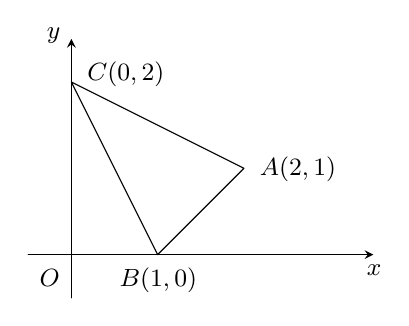
\begin{tikzpicture}[x=0.03515cm,y=0.03515cm,>=stealth,every node/.style={font=\small,inner sep=0pt},
  gl/.style={line width=0.398bp,line cap=round,line join=round}]
% ===== 坐标轴（单向箭头，照源顶点）=====
\draw[gl,->] (-15.5859,0)--(109.0938,0);   % x 轴
\draw[gl,->] (0,-15.5820)--(0,77.9258);    % y 轴
% ===== 三角区域（闭合实线）=====
\draw[gl] (0,62.3398)--(62.3399,31.1719)--(31.1680,0)--cycle;
% ===== 标签（照源字形包围盒中心定位）=====
\node at (-6.4434,79.1703) {\(y\)};
\node at (19.6966,65.3103) {\(C(0,2)\)};
\node at (81.8666,31.0103) {\(A(2,1)\)};
\node at (109.3416,-5.7647) {\(x\)};
\node at (-7.7934,-8.4197) {\(O\)};
\node at (31.3866,-9.1197) {\(B(1,0)\)};
\end{tikzpicture}
